%\documentclass{exam}

\usepackage[hangul]{kotex} %<===> EUC-KR
\usepackage{ifxetex} % 부득이하게 pdflatex을 사용해도 문제가 없도록 함

\ifxetex
%한글 사용 옵션
\RequirePackage{xetexko}
\setmainfont[Ligatures=TeX]{Batang}
\setmainhangulfont[BoldFont=*,BoldFeatures=FakeBold,%
ItalicFont=*,ItalicFeatures=FakeSlant]{Batang}
\disablecjksymbolspacing
\nonfrenchspacing
\else
\fi

\usepackage[T1]{fontenc}
\usepackage{pslatex}
\usepackage[pdftex]{color}  
\usepackage[pdftex]{graphicx}     

\usepackage{titlesec}
\usepackage{verbatim}
\usepackage[title,titletoc]{appendix}
\usepackage{booktabs}
\usepackage{graphicx}
\usepackage{tikz}
\usepackage{setspace}
\usepackage{amssymb}
\usepackage{bigstrut}
\usepackage{lineno}
\usepackage{afterpage}
\usepackage{graphicx}
\usepackage{array}
\usepackage{multirow}
\usepackage{amsfonts,epsfig}
\usepackage{rotating}
\usepackage{algorithmicx}
\usepackage{color}
\usepackage{subcaption}
\captionsetup{compatibility=false}
\usepackage[normalem]{ulem}
\usepackage{pstricks,pst-node,amsmath}
\usepackage{multirow}
\usepackage{graphicx,amsmath} 
\usepackage{flushend}
\usepackage{amssymb,amsfonts,amsbsy,epsfig}
\usepackage{lscape}
\usepackage[noend]{algpseudocode}
\usepackage{epstopdf}
\usepackage{amsmath,mathtools}
\usepackage{framed}
\usepackage{algorithm}
\usepackage{hyperref}
\usepackage[margin=0.5 in]{geometry}
\usepackage[symbol]{footmisc}
\usepackage [english]{babel}
\usepackage [autostyle, english = american]{csquotes}
\MakeOuterQuote{"}
\usepackage{amssymb}
\usepackage{xspace}
\usepackage{setspace}
\usepackage{array}
\usepackage{textcomp}

\begin{document}
	%----------------------------------------------------------------------------------------
%	SECTION 1
%----------------------------------------------------------------------------------------
\section{유효 온도 (effective temperature)}

\pagestyle{headings}
\markboth{유효 온도 (effective temperature)\hfill Kiehyun Park\hfill}

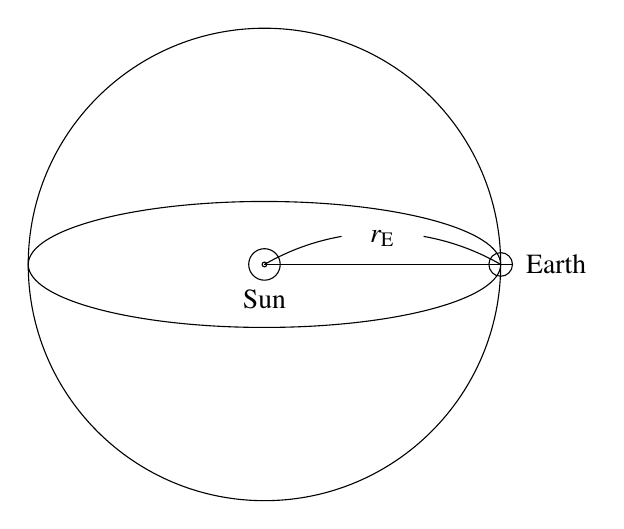
\begin{tikzpicture}[scale = 1, xshift = 1cm]
	\draw (5,2) circle (3cm);
	\draw (5,2) ellipse (3cm and 0.8cm);
	\draw (5,2) circle (0.03cm);
	\draw (5,2) circle (0.2cm) node[below, yshift=-0.2cm] {Sun};
	\draw (8,2) circle (0.15cm) node[right, xshift=0.2cm] {Earth};
	\draw (5,2) -- (8,2) node[above, xshift=-1.5cm, yshift=0.1cm] {$r_{\mathrm{E}}$};
	\draw (5,2) arc (120:100:3cm);
	\draw (8,2) arc (60:80:3cm);
	\draw (7.85,2) -- (8.15,2);
	\draw (8,1.85) -- (8,2.15);
\end{tikzpicture}

\vspace{1cm}
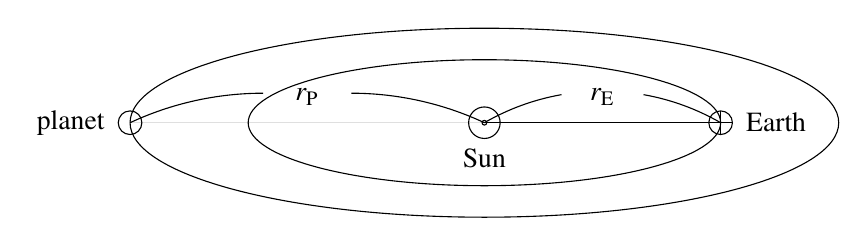
\begin{tikzpicture}[scale = 1, xshift = 1cm]
	\draw (5,2) ellipse (3cm and 0.8cm);
	\draw (5,2) ellipse (4.5cm and 1.2cm);
	\draw (5,2) circle (0.03cm);
	\draw (5,2) circle (0.2cm) node[below, yshift=-0.2cm] {Sun};
	\draw (8,2) circle (0.15cm) node[right, xshift=0.2cm] {Earth};
	\draw (5,2) -- (8,2) node[above, xshift=-1.5cm, yshift=0.1cm] {$r_{\mathrm{E}}$};
	\draw (5,2) arc (120:100:3cm);
	\draw (8,2) arc (60:80:3cm);
	\draw (0.5,2) circle (0.15cm) node[left, xshift=-0.2cm] {planet};
	\fill (5,2) -- (0.5,2) node[above, xshift=2.25cm, yshift=0.1cm] {$r_{\mathrm{P}}$};
	\draw (0.5,2) arc (115:90:4cm);
	\draw (5,2) arc (65:90:4cm);
	\draw (7.85,2) -- (8.15,2);
	\draw (8,1.85) -- (8,2.15);
\end{tikzpicture} 
	
\vspace{1cm}
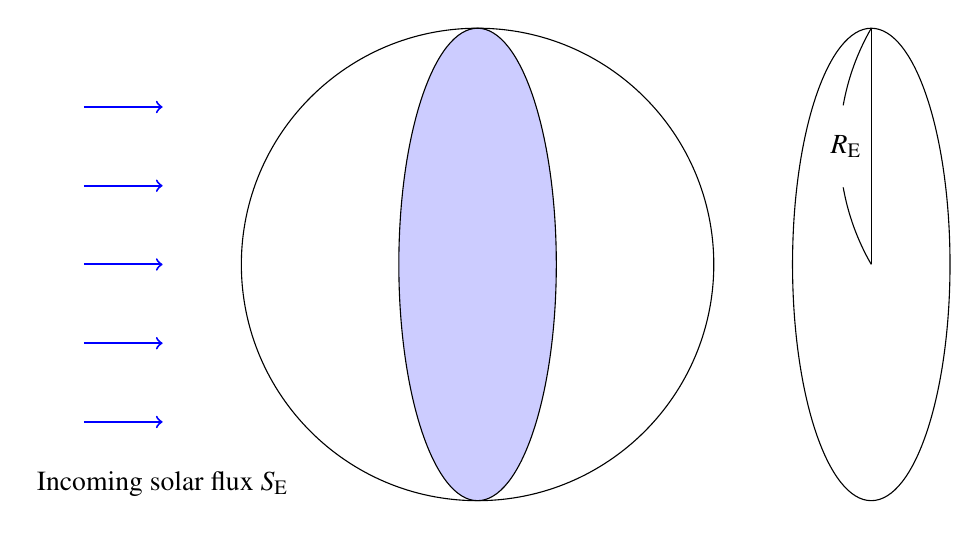
\begin{tikzpicture}[scale = 1, xshift = 1cm]
	\draw [line width=0.25mm, blue] [->] (0,0) -- (1,0) node[black, below, yshift=-0.5cm] {Incoming solar flux $S_{\mathrm{E}}$};
	\draw [line width=0.25mm, blue] [->] (0,1) -- (1,1);
	\draw [line width=0.25mm, blue] [->] (0,2) -- (1,2);
	\draw [line width=0.25mm, blue] [->] (0,3) -- (1,3);
	\draw [line width=0.25mm, blue] [->] (0,4) -- (1,4) ;
	
	\draw (5,2) circle (3cm);
	
	\fill [blue!20!white] (5,2) ellipse (1cm and 3cm) ;
	\draw (5,2) ellipse (1cm and 3cm) ;
	\draw (10,2) ellipse (1cm and 3cm);
	\draw (10,2) -- (10,5) node[left, yshift=-1.5cm] {$R_{\mathrm{E}}$};
	\draw (10,2) arc (210:190:3cm);
	\draw (10,5) arc (150:170:3cm);
\end{tikzpicture}


\begin{figure*}[h]
	\begin{tikzpicture}[rounded corners=3mm]
	\path node[rectangle,draw=green,fill=green!8,inner sep=.70cm] 
	{\parbox[t][15.5cm]{\textwidth-1.4cm-\fboxrule}
		{\question 
			* 행성의 유효 온도를 구하시오.
			\begin{solutionorlines}[15cm]

			* 지구에서의 태양 상수는
			$S_{\mathrm{E}} = \dfrac{L_{\odot}}{4\pi r_{\mathrm{E}}^{2}}$

			* 행성의 태양 상수($ S_{\mathrm{P}}$)와 지구의 태양 상수 $S_{\mathrm{E}}$는 
			$ S_{\mathrm{P}} = S_{\mathrm{E}}\left(\dfrac{r_{\mathrm{E}}}{r_{\mathrm{P}}}\right)^{2}$
			
			* 지구가 받는 태양 복사 에너지는  
			$\pi R_{\mathrm{E}}^{2} S_{\mathrm{E}}$

			* 행성이 받는 태양 복사 에너지는 
			$ \pi R_{\mathrm{P}}^{2} S_{\mathrm{E}}\left(\dfrac{r_{\mathrm{E}}}{r_{\mathrm{P}}}\right)^{2}$
			
			* 알베도($A$)를 고려하면 
			$ I_{\mathrm{P}}^{\downarrow} = (1-A)\pi R_{\mathrm{P}}^{2} S_{\mathrm{E}}\left(\dfrac{r_{\mathrm{E}}}{r_{\mathrm{P}}}\right)^{2}$
			
			* Stefan-Boltzmann 법칙에 따라 행성이 방출하는 복사 에너지량은
			$ I_{\mathrm{P}}^{\uparrow} = 4\pi R_{\mathrm{P}}^{2} \sigma T^{4}$
			
			* 따라서 행성의 유효 온도는
			$ T_{e} = \sqrt[4]{\dfrac{(1-A) S_{\mathrm{E}}}{4 \sigma}} \sqrt{\dfrac{r_{\mathrm{E}}}{r_{\mathrm{P}}}} $
			
			유효 온도는 행성과 태양과의 거리, 알베도에 의해 결정되며 대기의 구성 성분이나 밀도 등의 물리적 성질과는 무관하다.
			
			그러나 실제로 대기를 투과한 태양광이 대기의 구성 성분이나 지면에 흡수되고, 또 재방출 되는 복잡한 과정을 통하여 온도가 결정되므로 이러한 온도를 복사 온도(radiative temperature)라 한다. 
			실제 표면 온도는 행성의 유효온도에 대기의 온실효과 등이 더해져서 결정되어진 온도이다. 
			\end{solutionorlines}
	}};
	\end{tikzpicture}
\end{figure*}


\end{questions}
%(https://solarsystem.nasa.gov/system/resources/detail_files/681_ptemp.jpg)	
\section{이탈 속도 (escape velocity)}

\pagestyle{headings}
\markboth{이탈 속도 (escape velocity)\hfill Kiehyun Park\hfill}



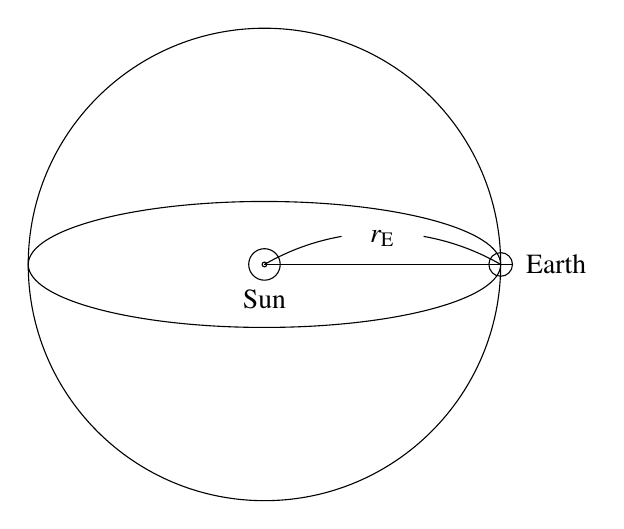
\begin{tikzpicture}[scale = 1, xshift = 1cm]
	\draw (5,2) circle (3cm);
	\draw (5,2) ellipse (3cm and 0.8cm);
	\draw (5,2) circle (0.03cm);
	\draw (5,2) circle (0.2cm) node[below, yshift=-0.2cm] {Sun};
	\draw (8,2) circle (0.15cm) node[right, xshift=0.2cm] {Earth};
	\draw (5,2) -- (8,2) node[above, xshift=-1.5cm, yshift=0.1cm] {$r_{\mathrm{E}}$};
	\draw (5,2) arc (120:100:3cm);
	\draw (8,2) arc (60:80:3cm);
	\draw (7.85,2) -- (8.15,2);
	\draw (8,1.85) -- (8,2.15);
\end{tikzpicture}

\vspace{1cm}
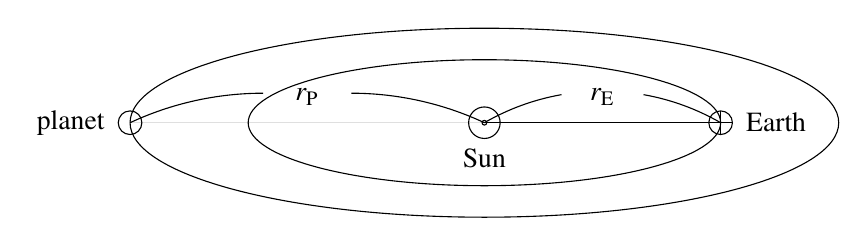
\begin{tikzpicture}[scale = 1, xshift = 1cm]
	\draw (5,2) ellipse (3cm and 0.8cm);
	\draw (5,2) ellipse (4.5cm and 1.2cm);
	\draw (5,2) circle (0.03cm);
	\draw (5,2) circle (0.2cm) node[below, yshift=-0.2cm] {Sun};
	\draw (8,2) circle (0.15cm) node[right, xshift=0.2cm] {Earth};
	\draw (5,2) -- (8,2) node[above, xshift=-1.5cm, yshift=0.1cm] {$r_{\mathrm{E}}$};
	\draw (5,2) arc (120:100:3cm);
	\draw (8,2) arc (60:80:3cm);
	\draw (0.5,2) circle (0.15cm) node[left, xshift=-0.2cm] {planet};
	\fill (5,2) -- (0.5,2) node[above, xshift=2.25cm, yshift=0.1cm] {$r_{\mathrm{P}}$};
	\draw (0.5,2) arc (115:90:4cm);
	\draw (5,2) arc (65:90:4cm);
	\draw (7.85,2) -- (8.15,2);
	\draw (8,1.85) -- (8,2.15);
\end{tikzpicture} 
	
\vspace{1cm}
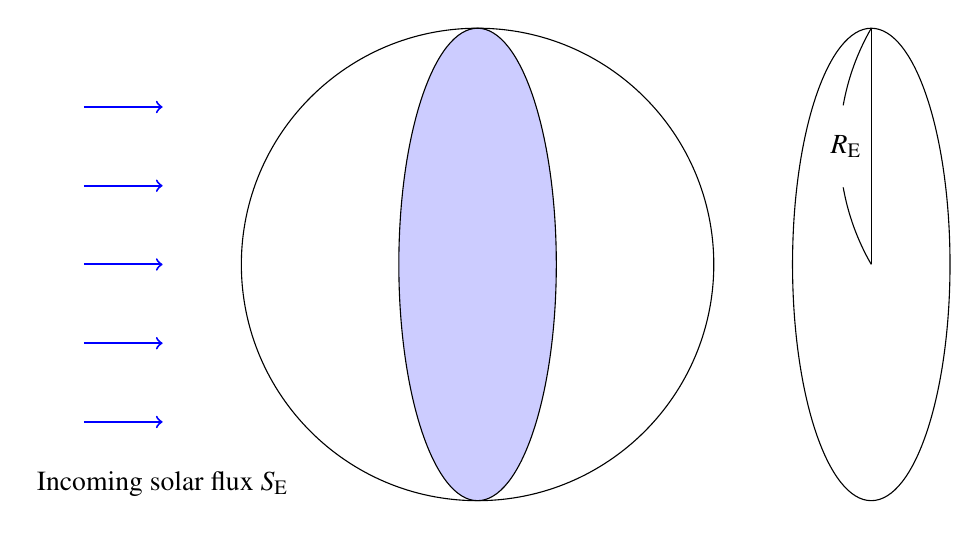
\begin{tikzpicture}[scale = 1, xshift = 1cm]
	\draw [line width=0.25mm, blue] [->] (0,0) -- (1,0) node[black, below, yshift=-0.5cm] {Incoming solar flux $S_{\mathrm{E}}$};
	\draw [line width=0.25mm, blue] [->] (0,1) -- (1,1);
	\draw [line width=0.25mm, blue] [->] (0,2) -- (1,2);
	\draw [line width=0.25mm, blue] [->] (0,3) -- (1,3);
	\draw [line width=0.25mm, blue] [->] (0,4) -- (1,4) ;
	
	\draw (5,2) circle (3cm);
	
	\fill [blue!20!white] (5,2) ellipse (1cm and 3cm) ;
	\draw (5,2) ellipse (1cm and 3cm) ;
	\draw (10,2) ellipse (1cm and 3cm);
	\draw (10,2) -- (10,5) node[left, yshift=-1.5cm] {$R_{\mathrm{E}}$};
	\draw (10,2) arc (210:190:3cm);
	\draw (10,5) arc (150:170:3cm);
\end{tikzpicture}

\begin{figure*}[h]
	\begin{tikzpicture}[rounded corners=3mm]
	\path node[rectangle,draw=green,fill=green!8,inner sep=.70cm] 
	{\parbox[t][15.5cm]{\textwidth-1.4cm-\fboxrule}
		{\question 
			행성 표면으로부터 고도 $h$에 있는 단위 질량인 물체의 이탈 속도를 구하시오.
			\begin{solutionorlines}[15cm]
			* 중력으로부터 물체가 탈출하는데 필요한 속도를 이탈 속도라고 하며 다음과 같이 구할 수 있다. 

			$ \dfrac{1}{2} m v_{\mathrm{e}}^{2} + \dfrac {- G M m}{r} = 0 $

			행성 대기의 상층부는 기체의 밀도가 낮으므로, 분자와 원자가 다른 분자나 원자와 충돌할 확률이 매우 적다 따라서 평균자유행로가 크며, 커다란 운동에너지를 가지므로 속도가 빨라 생성의 중력으로 부터 벗어나 외계로 이탈할 수 있다. 

			*   행성 표면으로부터 고도 $h$에 있는 단위 질량인 물체의 이탈 속도 : 

			$ v_{\mathrm{e}} = \sqrt {\dfrac{2Gm_{\mathrm{p}}}{r_{\mathrm{p}} + h}} $
			($G = 6.668\times10^{-11}\mathrm{kg^{-11} m^{3} s^{-2}}$)

			기체 분자에 이탈속도를 적용해 보자. 
			\end{solutionorlines}
	}};
	\end{tikzpicture}
\end{figure*}

\end{questions}

%(https://solarsystem.nasa.gov/system/resources/detail_files/681_ptemp.jpg)

# 맥스웰-볼츠만 분포

기체 분자들이 운동하고 있을 때 속도에 따른 분자 갯수는 맥스웰-볼츠만 분포를 따르게 되는데 이는 어떤 기체분자가 속도($v$)를 가질 확률이다. 

![대체 텍스트](http://www.kshitij-iitjee.com/Study/Physics/Part3/Chapter21/79.jpg)

위 그림을 보면 낮은 온도에서(파랑) 느린 분자가 압도적으로 많고, 빠른 기체분자는 거의 없다. 
높은 온도에서는(빨강) 빠른 분자가 많지만, 훨씬 완만한 분포를 가지며 느린 분자도 여전히 존재한다. 

분자들의 속력에 대한 멕스웰-볼츠만 분포는 아래와 같이 쓸 수 있다.

$f(v) = 4 \pi \left(\frac{M}{2\pi R T} \right)^{\dfrac{3}{2}} v^2 ~\mathrm{exp}\it \left[\dfrac{-Mv^2}{\rm{2} \it RT}\right]$

$f(v) = 4 \pi \left(\frac{m}{2\pi k T} \right)^{\dfrac{3}{2}} v^2 ~\mathrm{exp}\it \left[\dfrac{-mv^2}{\rm{2} \it kT}\right]$

($M$: 분자량, $m$: 분자의 질량)

최빈 속력($v_{\mathrm{mp}}$)는 $\dfrac{df(v)}{dv} = 0$으로 두고 $v_{mp}$에 대하여 풀어보자.

$\dfrac{d f(v)}{d v}=4 \pi\left(\dfrac{m}{2 \pi k T}\right)^{\frac{3}{2}}\left(2 v e^{\frac{-m v^{2}}{2 k T}}+\dfrac{-2 m v}{2 k T} v^{2} e^{\frac{-m v^{2}}{2 k T}}\right)$

$=4 \pi\left(\dfrac{m}{2 \pi k T}\right)^{\frac{3}{2}} v e^{\frac{-m v^{2}}{2 k T}}\left(2-\dfrac{m}{k T} v^{2}\right)=0$

$2-\dfrac{m}{k T} v^{2} = 0$, $v_{\mathrm{mp}} =  \sqrt {\dfrac{2kT}{m}} $, $v_{\mathrm{mp}} = \sqrt {\dfrac{2RT}{M}} $

평균 속력은 속력 분포의 수학적 평균이므로 다음과 같이 된다.

$${\overline{v}} = \int_{0}^{\infty} v f(v) dv$$

이를 부분 적분을 이용해 보자.
$$\left(\int f(x) g^{\prime}(x) d x=f(x) g(x)-\int f^{\prime}(x) g(x) d x\right)$$

$$\int_{0}^{\infty} x^{3} e^{-x^{2}} d x=\dfrac{1}{2}$$

$$\int_{0}^{\infty} x^{4} e^{-x^{2}} d x=\dfrac{1}{2}$$

임을 보이자.

$$\int_{0}^{\infty} x^{3} e^{-x^{2}} d x=\left[-\frac{x^{2}}{2} e^{-x^{2}}\right]_{0}^{\infty}+\int_{0}^{\infty} x e^{-x^{2}} dx \\
$=\left[-\frac{x^{2}}{2} e^{-x^{2}}\right]_{0}^{\infty}-\left[\dfrac{1}{2} e^{-x^{2}}\right]_{0}^{\infty} \\
=\lim_{y \rightarrow \infty}\left(-\dfrac{y^{2}}{2} e^{-y^{2}}-\dfrac{1}{2} e^{-y^{2}}\right)+\dfrac{1}{2} = \dfrac{1}{2}$\\

$ {\overline{v}} = \sqrt {\dfrac{8kT}{\pi m}} \\
{\overline{v}} = \sqrt {\dfrac{8RT}{\pi M}}$


또한 제곱 평균 속도, $v_{rms}$는 속력에 제곱하여 평균한 값에 제곱근을 취한 것이기 때문에 밑의 식으로 나타낼 수 있다.


$v_{\mathrm {rms} } = \sqrt {{\int _{0}^{\infty }v^{2}\, f(v)\, dv}} $

$v_{\mathrm {rms} }={\sqrt {\dfrac {3RT}{M}}}$, $v_{\mathrm {rms} } = {\sqrt {\dfrac {3kT}{m}}}$


따라서 전체 속력은 아래와 같다.

$v_{\mathrm{mp}}<\overline{v} <v_{\mathrm {rms} }$


# 기체 분자 운동론

이상 기체를 가정하고 기체분자를 $x$, $y$, $z$ 방향중 $x$방향의 운동만 고려하면아래와 같이 모식할 수 있다.

![대체 텍스트](https://encrypted-tbn0.gstatic.com/images?q=tbn:ANd9GcRsHZTF-U5SpCHv93NAmYHiyoM8NwH9fKybymRd96oHcbaPhoFs)

$\Delta t$의 시간 동안 기체분자가 $2L$의 거리를 움직이므로 속도 $v$와 $\Delta t$는

$ v = \dfrac{2L}{\Delta t} $, $\Delta t = {2L}{v}$

완전탄성충돌을 가정했으므로 속도는 방향이 반대이고 크기가 같다. 따라서 운동량변화량은 

$\Delta P = mv - (-mv) = 2mv$

힘의 정의에서 다음과 같이 정리된다.

$F = \dfrac{\Delta P}{Delta t} = \dfrac{2mv}{\dfrac{2L}{v}} = \dfrac{2mv^2}{L}$

또한 압력의 정의에서

$ pressure = \dfrac{force}{area} = \dfrac{\dfrac{mv^2}{L}}{L^2} = \dfrac{mv^2}{L^3} = \dfrac {mv^2}{volume}$

1몰의 기체에 대해서는 아보가드로수를 곱해주고 보편기체상수$R$ 나누기 아보가드로수 $N_a$는 볼츠만 상수 $k$ 이므로 이상기체가정에 따라
$Pressure \times volyme = nRT - N_{A} mv^2$
$kT = mv^2$

운동에너지 정의에서

$E_{k, x} = \dfrac{1}{2} mv^2 = \dfrac{1}{2} kT$

분자는 $x$, $y$, $z$ 세 방향 모두 고려해주면
$E_{k} = E_{k, x} + E_{k, y} + E_{k, z} = \dfrac{3}{2} kT$

단원자기체가 아닌경우 분자의 회전운동을 고려해줘야 하기때문에

단원자 : $\dfrac{3}{2} kT$

이원자 : $\dfrac{5}{2} kT$

다원자 : $\dfrac{7}{2} kT$



# 이상 기체 상태 방정식

거시적인 이상 기체 상태 방정식은 다음과 같은 식으로 표현된다. 

*  $ PV = nRT $
($P$:압력, $V$:부피, $n$:기체의 몰수, $R$:기체 상수, $T$: 절대 온도)

실제 기체는 근사적으로 대개 이상 기체 법칙을 따르며, 기체의 밀도가 0에 가깝거나 기체의 온도가 매우 높으면 이상 기체 법칙에 더 잘 맞게 된다. 그 이유는 밀도가 0에 가까워지면 분자의 운동시 기체 분자끼리 부딪히는 정도가 적어지고 분자 자신의 부피를 무시할 정도가 된다. 또 고온이 됨으로써 분자의 운동이 고속이 되어 분자 간의 힘이 무시할 만한 정도가 되기 때문이다.

이를 미시적 관점에서 본 미시적인 이상 기체 법칙은 다음과 같다.

*  $ PV = N k T $
($P$:압력, $V$:부피, $N$:기체의 분자수, $k$:볼츠만 상수, $T$:절대 온도)

*  $ R = \dfrac{Nk}{n} $



# 행성의 대기


![대체 텍스트](http://ircamera.as.arizona.edu/astr_250/images/esc_vel.gif)

![대체 텍스트](https://i2.wp.com/mathscinotes.com/wp-content/uploads/2016/08/MolecularEscapeVelocity1.png)

기체분자론에 의하면 평균 분자 속도 ${\overline{v}}$ 가 갖는 운동에너지는 기체의 운동학적 온도 $T_{k}$ (kinetic temperature)와 분자의 질량($nm$)에 의해서 결정되므로 다음과 같이 나타낼 수 있다.

*  $ \dfrac{1}{2} m {\overline{v}}^{2} = \dfrac{3}{2} k T_{k}$

*  $ \overline{v} = \sqrt {\dfrac{3kT_{k}}{m}} $
($m$: 기체분자 1개의 질량, $k = 1.380658 \times 10^{23}\rm{J K^{-1}}$) 









	
\section{대기역학}

\sebsection{압력 경도력}


두 지점 사이의 압력 차이에 의해 압력이 큰 쪽에서 작은 쪽으로 압력 경도력이 작용한다. 대기에서는 기압 경도력, 해수에서는 수압 경도력으로 작용한다


같이 세 변이 각각 Dx, Dy , Dz로 이루어진 육면체를 고려하자. 이 육면체의 왼쪽 A면에
작용하는 평균기압을 p라고 하면 A면에 작용하는 힘의 크기는 pDyDz이고 방향은 +x방향이다. 육면체에서
왼쪽에서 오른쪽으로 기압이 Dp만큼 증가한다면 B면에 작용하는 기압의 크기는 ( p+Dp )DyDz이고
방향은 -x방향이다. 이 육면체에 작용하는 기압력의 x성분인 Fx 는 A와 B면에 작용하는 힘들의 합이므로,


#좌표계1

관성계 : 절대 좌표계 $ (x,~y,~z)$

비관성계 : 회전 좌표계 $ (x^{\prime},~y^{\prime},~z^{\prime})$ 

극좌표 $ (r,~\theta,~z)$


$ (x,~y,~z) 	\rightarrow (r,~\theta,~z)$ 
에서 수평 방향은 정역학 평형 상태에 있으므로, 

$ (x, y) 	\rightarrow (r, \theta)$

>$ \mathbf{F} = F_{x} \mathbf{\hat{i}}  + F_{y} \mathbf{\hat{j}} $ 
에서 

>$ F_{x} = m \dfrac{d^{2}x}{dt^{2}}$, 
>$ F_{y} = m \dfrac{d^{2}y}{dt^{2}}$ 

라고 할 수 있다. 

>$ (x, y) = (r \cos \theta, r \sin \theta)$ 

에서

>$ F_{r} = F_{x} \cos \theta + F_{y} \sin \theta $, 

>$ F_{\theta} = F_{y} \cos \theta - F_{x} \cos \theta $ 

로 나타낼 수 있다. 

>$ x = r \cos \theta $

를 미분하면, 

>$\dfrac{dx}{dt} = \cos \theta \dfrac{dr}{dt} - r \sin \theta \dfrac{d\theta}{dt}$ 

이고, 이를 다시 미분하면, 

> $\dfrac{d^{2}x}{dt^{2}} = \cos \theta \dfrac{d^{2}r}{dt^{2}} - \sin \theta \dfrac{dr}{dt} - \sin \theta \dfrac{dr}{dt} \dfrac{d\theta}{dt} -r \cos \theta \dfrac{d^{2}\theta}{dt^{2}}$

같은 방법으로 
>$ y = r \sin \theta $ 

를 미분하면
>$\dfrac{dy}{dt} = \sin \theta \dfrac{dr}{dt} + r \cos \theta \dfrac{d\theta}{dt}$ 

이고, 이를 다시 미분하면

>$\dfrac{d^{2}t}{dt^{2}} = \sin \theta \dfrac{d^{2}r}{dt^{2}} + \cos \theta \dfrac{dr}{dt} + \cos \theta \dfrac{dr}{dt} \dfrac{d\theta}{dt} -r \sin \theta \dfrac{d^{2}\theta}{dt^{2}}$

이다. 

>$ F_{r} = F_{x} \cos \theta + F_{y} \sin \theta 
= m \left ( \dfrac{d^{2}x}{dt^{2}} \cos \theta + \dfrac{d^{2}y}{dt^{2}} \sin \theta \right) $

>$ F_{\theta} = F_{y} \cos \theta - F_{x} \cos \theta 
= m \left ( \dfrac{d^{2}y}{dt^{2}} \cos \theta - \dfrac{d^{2}x}{dt^{2}} \cos \theta \right) $


정리하면, 

> $ F_{r} = m \left[ \dfrac{d^{2}r}{dt^{2}} - r \left( {\dfrac{d \theta}{dt}} \right)^{2} \right] $에서,

>$ -r \left( {\dfrac{d \theta}{dt}} \right)^{2} \rightarrow $ Centrifugal force \\

>$ F_{\theta} = m \left[ r \dfrac{d^{2}\theta}{dt^{2}} + 2 \dfrac{dr}{dt} \dfrac{d\theta}{dt}  \right] $에서, 

>$ 2 \dfrac{dr}{dt} \dfrac{d\theta}{dt} \rightarrow $ Coriolis force \\




#좌표계2

$ (x,~y) 	\rightarrow (x^{\prime},~y^{\prime})$

>$ \mathbf {F} = F_{x} \mathbf{\hat{i}} + F_{y} \mathbf{\hat{j}} $

에서 

>$ F_{x} = m \dfrac{d^{2}x}{dt^{2}}$, 

>$ F_{y} = m \dfrac{d^{2}y}{dt^{2}}$ 

라고 할 수 있다.

>$ x^{\prime} = x \cos \omega t + y \sin \omega t$, 

>$ y^{\prime} = -x \sin \omega t + y \cos \omega t$

>$ \mathbf {F} = F_{x^{\prime}} \mathbf {\hat{i}}  + F_{y^{\prime}} \mathbf {\hat{j}} $

>$ F_{x^{\prime}} = F_{x} \cos \omega t + F_{y} \sin \omega t
= m \left ( \dfrac{d^{2}x}{dt^{2}} \cos \omega t + \dfrac{d^{2}y}{dt^{2}} \sin \omega t \right) $

>$ F_{y^{\prime}} = -F_{x} \sin \omega t + F_{y} \cos \omega t
= m \left ( - \dfrac{d^{2}x}{dt^{2}} \sin \Omega t + \dfrac{d^{2}y}{dt^{2}} \cos \omega t \right) $

정리하면,

>$ F_{x^{\prime}} = m \left( \dfrac{d^{2}x}{dt^{2}}F_{x} - 2 \omega  \dfrac{dy}{dt} - 2 \omega^{2} x^{\prime}  \right) $

>$ F_{y^{\prime}} = m \left( \dfrac{d^{2}y}{dt^{2}}F_{x} + 2 \omega  \dfrac{dx}{dt} - 2 \omega^{2} y^{\prime}  \right) $

추가 작성 필요함...


# Pressure gradient force

>$ dV = dx \cdot dy \cdot dz $


$x$ 방향은

>$ F_{x} = P \cdot \Delta y \cdot \Delta z - \left( P + \Delta P \right) \Delta y \cdot \Delta z$

>$ F_{x} = - \Delta P \cdot \Delta y \cdot \Delta z $

>$ \dfrac { \Delta y}{\Delta x } = \dfrac {f\left(x + \Delta x \right) - f\left(x \right)}{ \Delta x}$

>$f^{\prime} \left(x \right) = lim \dfrac { \Delta y}{\Delta x } 
= \dfrac {f\left(x + \Delta x \right) - f\left(x \right)}{ \Delta x}$


>$z = f \left( x, y \right) $ 

에서 $y = b \rightarrow b$ 를 고정 하고 $x$ 방향에 대해서만 극한을 취하는 것을 편미분이라 한다.

>$ \displaystyle \lim_{\Delta x \rightarrow 0} \dfrac { \Delta z}{\Delta x } 
= \dfrac {f\left(x + \Delta x, b \right) - f\left(x, b \right)}{ \Delta x} = \dfrac{\partial z}{\partial x} $

>$\displaystyle \lim_{\Delta y \rightarrow 0} \dfrac { \Delta z}{\Delta y } 
= \dfrac {f\left(y + \Delta y, b \right) - f\left(y, b \right)}{ \Delta y} = \dfrac{\partial z}{\partial y} $

>$ \Delta z = \dfrac{\partial z}{\partial x} \Delta x + \dfrac{\partial z}{\partial y} \Delta y $

>$ dz = \dfrac{\partial z}{\partial x} dx + \dfrac{\partial z}{\partial y} dy $

라고 쓸 수 있다.

>$ F_{x} = - \Delta P \cdot \Delta y \cdot \Delta z 
= \dfrac{\partial P}{\partial x} \cdot \Delta x \cdot \Delta y \cdot \Delta z $

>$ F_{y} = - \Delta P \cdot \Delta z \cdot \Delta x 
= \dfrac{\partial P}{\partial y} \cdot \Delta x \cdot \Delta y \cdot \Delta z $

>$ F_{z} = - \Delta P \cdot \Delta x \cdot \Delta y 
= \dfrac{\partial P}{\partial z} \cdot \Delta x \cdot \Delta y \cdot \Delta z $

>$ \rho = \dfrac {m}{\Delta x \cdot \Delta y \cdot \Delta z} $ 

단위 질량당 작용하는 각각의 힘은

>$ \dfrac {F_{x}}{m} = - \dfrac{1}{\rho} \dfrac{\partial P}{\partial x} $ 
>$ \dfrac {F_{y}}{m} = - \dfrac{1}{\rho} \dfrac{\partial P}{\partial y} $ 
>$ \dfrac {F_{z}}{m} = - \dfrac{1}{\rho} \dfrac{\partial P}{\partial z} $ 

이므로 단위질량당 기압경도력은 다음과 같이 쓸 수 있다.

>$ \dfrac {F}{m} = - \dfrac{1}{\rho} \left( \dfrac{\partial P}{\partial x} i + \dfrac{\partial P}{\partial y} j + \dfrac{\partial P}{\partial z} k \right) 
= - \dfrac{1}{\rho} \nabla P$ 

# 회전계에서의 운동 방정식

온도를 자동으로 측정하여 무선으로 송신하는 장치를 대형 풍선에 매달아 날려보낸다고 하자.

시각 $ t_{o}$, 위치 $(x_{o},~y_{o},~z_{o})$에서 측정된 온도를 $T_{o}$라 하자. 

시각 $ t_{o}+\Delta t$, 위치 $(x_{o}+\Delta x,~y_{o}+\Delta y,~z_{o}+\Delta z)$에서 측정된 온도를 $T_{o}+\Delta T$ 라고 하면

>$ \Delta T = \dfrac{\partial T}{\partial t} \Delta t 
+ \dfrac{\partial T}{\partial x} \Delta x 
+ \dfrac{\partial T}{\partial y} \Delta y 
+ \dfrac{\partial T}{\partial z} \Delta z $

이 식을 $ \Delta T $로 나누고 0으로 극한을 취하면,

>$ \displaystyle \lim_{\Delta t \rightarrow 0} \dfrac{\Delta T}{\Delta t} 
= \dfrac{DT}{Dt} = \dfrac{\partial T}{\partial t} 
+ \dfrac{\partial T}{\partial x} \dfrac{Dx}{Dt}
+ \dfrac{\partial T}{\partial y} \dfrac{Dy}{Dt}
+ \dfrac{\partial T}{\partial z} \dfrac{Dz}{Dt} $

>$\dfrac{Dx}{Dt} \equiv u$, 
>$\dfrac{Dy}{Dt} \equiv v$, 
>$\dfrac{Dz}{Dt} \equiv w$, 

라고 정의하면


>$ \dfrac{DT}{Dt} = \dfrac{\partial T}{\partial t} 
+ \left( u \dfrac{\partial T}{\partial x}
+ v \dfrac{\partial T}{\partial y}
+ w \dfrac{\partial T}{\partial z} \right)
= \dfrac{\partial T}{\partial t} + U \cdot \nabla T $

여기에서 $ U = iu + jv + kw $ 3차원 속도 벡터 이다.

회전계에서의 운동방정식을 유도하면,

>$ \dfrac{DU}{Dt} = -2 \Omega \times U - \dfrac{1}{\rho} \nabla p + g + F_{r} $

와 같이 나타낼 수 있다.



# 직각 카테시안 좌표계에서의 운동 방정식

>$ \dfrac{DU}{Dt} = -2 \Omega \times U - \dfrac{1}{\rho} \nabla p + g + F_{r} $ 

에서, 먼저 전향력 성분을 나누어 보면, 

> $ \Omega_{x} = 0$,

> $ \Omega_{y} = \Omega \cos \phi$, 

> $ \Omega_{z} = \Omega \sin \phi$ 

이다.

> $ -2 \Omega \times U  
= -2 \left( 2 \Omega w \cos \phi -2 \Omega v \sin \phi \right) \mathbf{i}
- 2 \Omega u \sin \phi \mathbf{j}
+ 2 \Omega u \cos \phi \mathbf{k}$

로 나타낼 수 있다. 그리고 기압경도력을 나누어 보면, 

>$ \nabla p = \mathbf{i} \dfrac{\partial P}{\partial x} 
+ \mathbf{j} \dfrac{\partial P}{\partial y}
+ \mathbf{k} \dfrac{\partial P}{\partial z}$

중력은 

> $ \mathbf{g} = -g \mathbf{k} $

마찰력은

>$ F_{r} = \mathbf{i} F_{x}
+ \mathbf{j} F_{y}
+ \mathbf{k} F_{z}$

각 성분별로 운동방정식을 나타내면 

>$ \dfrac{Du}{Dt}
= - \dfrac{1}{\rho} \dfrac{\partial P}{\partial x} 
+ 2 \Omega v \sin \phi - 2 \Omega w \cos \phi 
+ F_{x} $

>$ \dfrac{Dv}{Dt}
= - \dfrac{1}{\rho} \dfrac{\partial P}{\partial x} 
- 2 \Omega u \sin \phi
+ F_{y} $

>$ \dfrac{Dw}{Dt}
= - \dfrac{1}{\rho} \dfrac{\partial P}{\partial x} 
+ 2 \Omega u \cos \phi 
+ F_{z}$

$x$ 성분에서 연직 전향력은 수평 전향력에 비해 매우 작은 값이므로, $- 2 \Omega w \cos \phi $ 항을 무시할 수 있다. 

$z$ 성분의 전향력 $ 2 \Omega u \cos \phi $ 은 중력 $g$에 비해 매우 작으므로 무시할 수 있다. 

더구나 $ \dfrac{Dw}{Dt}$의 크기는 더 작기 때문에 $ 2 \Omega \sin \phi $를 $f$로 두면 다음과 같이 간단히 할 수 있다.

>$ \dfrac{Du}{Dt}
= - \dfrac{1}{\rho} \dfrac{\partial P}{\partial x} 
+ 2 \Omega v \sin \phi 
= - \dfrac{1}{\rho} \dfrac{\partial P}{\partial x} 
+ f v $\\

>$ \dfrac{Dv}{Dt}
= - \dfrac{1}{\rho} \dfrac{\partial P}{\partial x} 
- 2 \Omega u \sin \phi
= - \dfrac{1}{\rho} \dfrac{\partial P}{\partial x}
- f u $\\

>$ 0
= - \dfrac{1}{\rho} \dfrac{\partial P}{\partial x} 
- g $



# 자연 좌표계

자연 좌표계 $ (s,~n,~z)$ 

* $ t $ : 유체가 움직이는 방향에 평행인 방향

* $ n $ : $ t $에 대하여 수직인 벡터이고 유체가 움직이는 방향의 왼쪽으로 향하는 방향이 + 방향임

* $ k $ : 연직 방향

>$\mathbf{V} = V \mathbf{t}$, $\mathbf{V} = \dfrac{Ds}{Dt}$

가속도는
>$ \dfrac{D\mathbf{V}}{Dt} = \mathbf{t} \dfrac{DV}{Dt} + V \dfrac{D \mathbf{t}}{Dt}$

>$ \Delta \Psi = \dfrac{\Delta V}{R}$ 이고, 

>$ \dfrac{D \mathbf{t}}{Ds} = \dfrac{\mathbf{n}}{R}$

따라서

>$ \dfrac{D \mathbf{t}}{Dt} = \dfrac{D \mathbf{t}}{Ds} \dfrac{Ds}{Dt} = \dfrac{\mathbf{n}}{R} V$

>$ \therefore \dfrac{D \mathbf{V}}{Dt} = \mathbf{t} \dfrac{DV}{Dt} + V \dfrac{D\mathbf{t}}{Dt} = \mathbf{t} \dfrac{DV}{Dt} + \mathbf{n} \dfrac{V^{2}}{R} $

전향력은 운동 방향의 오른쪽으로 작용하고 크기는 $fv$이므로 전향력은 $-f V \mathbf{n}$으로 나타내고, 

기압 경도력은 
>$ - \dfrac{1}{\rho} \left( \dfrac{\partial p}{\partial s} \mathbf{t} + \dfrac{\partial p}{\partial n} \mathbf{n} \right)$

로 나타낼 수 있다. 이 벡터 식을 s와 n 방향으로 나타내면

>$ \dfrac{D\mathbf{V}}{Dt} = - \dfrac{1}{\rho} \dfrac{\partial p}{\partial s}$

>$  \dfrac{V^{2}}{R} + fV = - \dfrac{1}{\rho} \dfrac{\partial p}{\partial n}$

등압선에 평행한 운동을 할 경우 공기덩이는 기압이 같은 곳으로 이동하므로

>$ \dfrac{\partial p}{\partial s} = 0 \rightarrow  \dfrac{DV}{Dt} = 0$





# 관성풍

>$  \dfrac{V^{2}}{R} + fV = 0$

>$ R = - \dfrac{V}{f} $

>$ P = \dfrac{2 \pi R}{V} =  \dfrac{2 \pi }{2 \Omega \sin \phi} =  \dfrac{1}{2}  \dfrac{day}{\sin \phi}$


# geostrophic wind

유체가 흐르는 방향에 평행한 방향과 수직인 방향 즉 자연좌표계에 대한 힘의 균형을 다음과 같이 나타낼 수 있다.

>$ \dfrac{D\mathbf{V}}{Dt} = - \dfrac{1}{\rho} \dfrac{\partial p}{\partial s}$

>$  \dfrac{V^{2}}{R} + fV = - \dfrac{1}{\rho} \dfrac{\partial p}{\partial n}$

지균풍의 경우에는 $\dfrac{\partial p}{\partial s} = 0$이고 등압선이 직선이므로 곡률반경 $R$의 절댓값은 $0$ 이 된다. 그러므로 지균풍은 아래와 같이 정의된다.

>$-f V_{g} = -\dfrac{1}{\rho}\dfrac{\partial p}{\partial n}$ 

지균풍의 풍속에 관해 정리하면

>$V_{g} = -\dfrac{1}{f \rho}\dfrac{\partial p}{\partial n}$ 



# 경도풍

>$  \dfrac{V^{2}}{R} + fV = - \dfrac{1}{\rho} \dfrac{\partial p}{\partial n}$

>$ V^{2} + fRV + \dfrac{R}{\rho} \dfrac{\partial p}{\partial n} = 0$

>$ V = -\dfrac{fR}{2} \pm \left( \dfrac{f^{2} R^{2}}{4} - \dfrac{R}{\rho}\dfrac{\partial p}{\partial n} \right)^{\dfrac{1}{2}} $ or $ - \dfrac{fR}{2} \pm \sqrt{ \dfrac{f^{2} R^{2}}{4} - \dfrac{R}{\rho}\dfrac{\partial p}{\partial n} }$



# 연습 문제 1. ~ 4.


-1. 질량이 1$\rm kg$인 공이 1$\rm m$ 줄에 매인 채로 마찰이 없는 수평면 위에서 2 $\rm rad ~ s^{-1}$ 의 속도로 회전하고 있다. 그런데 줄의 길이를 0.5 $\rm m$로 짧게 하여 회전시킬 때 

(1) 공의 회전 속도와 각운동량은 얼마가 되겠는가?

각운동량 보존법칙은 

>$ R_{1}~ V_{1} = R_{2}~ V_{2}$

> $ V_{1} = R_{1}~ \Omega_{1}$,  $ V_{2} = R_{2}~ \Omega_{2}$ 이므로

>$ {R_{1}}^{2}~ \Omega_{1} = {R_{2}}^{2}~ \Omega_{2}$

>$ {1}^2 \times 2 = {0.5}^2 \times \Omega_{2}$ 에서 

>$ \Omega_{2} = 8 \left( \rm rad ~ s^{-1} \right) $

회전 선속도는 
$ V_{2} = 0.5 \times 8 = 4 \left( \rm m ~ s^{-1} \right) $

각운동량은
$ {L}_{2} = R_{2} \times m V_{2} 
= 0.5 \cdot 1 \cdot 4 
= 2 \left( \rm kg ~ m^{2} ~ s^{-1} \right)$

이다.

(2) 구심 가속력은 얼마가 되겠는가?


구심 가속력은

>$ {R}_{2} ~ {\Omega}_{2}^{2}
= \cdot 0.5 \cdot 8^{2}
= 32 \left( \rm m ~ s^{-2} \right)$

-2.  북위  $37.5^{\circ}$에서 서풍이 5 $\rm m ~ s^{-1} $로 불고 있다. 절대 좌표계에서 이 바람을 관측하였다면 바람의 속도는 얼마가 되겠는가?

북위 $37.5^{\circ}$의 자전 선속도는

>$R_{E} \cdot \cos \phi \Omega
= 6380000 \cdot 0.7934 \cdot 7.29 \times 10^{-5}
= 369.01 \left( \rm m ~ s^{-1} \right)$


절대 좌표계에서 이 바람을 관측한다면 자전 선속도와 바람의 방향이 같으므로

>$369.01 + 5 = 374.01 \left( \rm m ~ s^{-1} \right)$ 이다.

-3.  북위  $30^{\circ}$에서 동쪽을 항하여 1000 $\rm km hr^{-1}$ 비행하는 비행기가 있다. 이 때 이 비행기에 타고 있는 사람(질량 65$\rm kg$)에게 작용하는 전향력을 구하여라.

전향력은 
>$ 2 m v \Omega \sin \phi
= \  2 \cdot 65 \cdot \dfrac{1000000} {3600} \cdot 7.29 \times 10^{-5} \cdot 0.5
= 1.32 \left( \rm kg~m ~ s^{-2} = N \right) $이다.

-4.  같은 위도대 (북위  $37^{\circ}$)에 있는 두 지역(100 $\rm km$ 떨어져 있음)의 기압차는 2 $\rm hPa$이다. 이 때 지균풍의 속력을 계산하라.

> $ f v_{g} = - {\rho} \dfrac{\partial P}{\partial n} $

에서, 지균풍의 풍속은 

>$ v_{g} = - \dfrac{1}{f \rho} \cdot \dfrac{\partial P}{\partial n}
= - \dfrac{1}{2 \Omega \sin \phi \rho~} \dfrac{\partial P}{\partial n} $
>$= - \cdot \dfrac{1}{2 \cdot 7.29 \times 10^{-5} \left( \rm s^{-1} \right) \cdot 0.5 \cdot \rho} \cdot \dfrac{200 \left( \rm kg~m~s^{-2} m^{-2} \right)} {100000 \left( \rm m \right)} 
= - \dfrac{1}{\rho} \cdot 27.43 \left( \rm kg~m^{-2}~ s^{-1} \right) $

이다. 공기의 밀도를 $ 1\rm kg~m^{-3}$이라고 가정하면, 

>$v_{g} = - 27.43 \left( \rm m~ s^{-1} \right) $

이다.



# 연습 문제 5. ~ 6.


-5. 북위  $30^{\circ}$에서 관성풍의 바람이 10 $\rm m s^{-1}$ 일 때, 관성원의 반지름은 얼마가 되겠는가?


관성원의 반지름은 

>$ R = - \dfrac{V}{f} = - \dfrac{V}{2 \Omega \sin \phi} = \dfrac{10}{2 \cdot 7.29 \times 10^{-5} \cdot 0.5} = 137,136.588 \left( \rm m \right) = 137.1 \left( \rm km \right)$

-6. 


경도풍은 다음과 같이 나타낼 수 있다.

>$ V^{2} + fRV + \dfrac{R}{\rho} \dfrac{\partial p}{\partial n} = 0$

지균풍은 

>$f V_{g} = -\dfrac{1}{\rho}\dfrac{\partial p}{\partial n}$ 

이므로 

>$V_{g} = -\dfrac{1}{f \rho}\dfrac{\partial p}{\partial n}$ 

>$ V^{2} + fRV - f R V_{g} = 0$


>$ V = -\dfrac{fR}{2} \pm \sqrt{ \dfrac{f^{2} R^{2}}{4} - \dfrac{R}{\rho}\dfrac{\partial p}{\partial n} } = -\dfrac{fR}{2} \pm \sqrt{ {\left(\dfrac{f R}{2} \right)}^{2} + f R V_{g} }$


저기압성 경도풍의 경우 $ R > 0$ 이고, $- \dfrac{\partial p}{\partial n} > 0$ 인 경우에 해당되므로, 

>$ V = -\dfrac{fR}{2} + \sqrt{ \dfrac{f^{2} R^{2}}{4} - \dfrac{R}{\rho}\dfrac{\partial p}{\partial n} } = -\dfrac{fR}{2} + \sqrt{ {\left(\dfrac{f R}{2} \right)}^{2} + f R V_{g} }$

>$ =  -\dfrac{ 2 \Omega \sin \phi R}{2} + \sqrt{ {\left(+\dfrac{ 2 \Omega \sin \phi R}{2} \right)}^{2} + 2 \Omega \sin \phi R V_{g} } $

>$ =  -\Omega \sin \phi R + \sqrt{ {\left(\Omega \sin \phi R \right)}^{2} + 2 \Omega \sin \phi R V_{g} } $

에서 

>$ \Omega \sin \phi R = 7.29 \times 10^{-5} \cdot 0.5 \cdot 1000000 =  36.45  \left( \rm m s^{-1} \right)$

이므로

>$ -\Omega \sin \phi R + \sqrt{ {\left(\Omega \sin \phi R \right)}^{2} + 2 \Omega \sin \phi R V_{g} }$

>$= -36.45+ \sqrt{ {\left(36.45 \right)}^{2} + 2 \cdot 36.45 \cdot 10 } $

>$ = -36.45+ 45.33 = 8.88 \left( \rm m s^{-1} \right)$




# 연습 문제 7. ~ 8. 


-7. 기압경도가 1000 $\rm km$당 10 $\rm hPa $이다. 이 때의 지균풍을 계산하라. 그리고 이러한 기압경도가 유지되면서, 곡률반경이 $\pm 500 \rm km$ 일 때의 경도풍들의 풍속을 계산하여 저기압의 경도풍이 지균풍보다 작음을 보이고, 반대로 고기압의 경도풍이 지균풍보다 큼을 보여라. 정상적인 경우와 비정상적인 경우 모두에 대하여 계산하라. $\rho = 1 \rm kg m^{-3}$ 이고, $ f = 10^{-4} s^{-1}$이다. 


지균풍은 

>$f V_{g} = -\dfrac{1}{\rho}\dfrac{\partial p}{\partial n}$ 

>$V_{g} = -\dfrac{1}{f \rho}\dfrac{\partial p}{\partial n} =  -\dfrac{1}{10^{-4} \cdot 1}\dfrac{-1000}{1000000} = 10 \left( \rm m s^{-1} \right)$ 

경도풍은 다음과 같이 나타낼 수 있다.

>$ V^{2} + fRV + \dfrac{R}{\rho} \dfrac{\partial p}{\partial n} = 0$

>$ V^{2} + fRV - f R V_{g} = 0$

>$ V = -\dfrac{fR}{2} \pm \sqrt{ \dfrac{f^{2} R^{2}}{4} - \dfrac{R}{\rho}\dfrac{\partial p}{\partial n} } = -\dfrac{fR}{2} \pm \sqrt{ {\left(\dfrac{f R}{2} \right)}^{2} + f R V_{g} }$

고기압성 경도풍은 $ R < 0$ 인 경우

>$ V_{GH} = -\dfrac{fR}{2} \pm \sqrt{ {\left(\dfrac{f R}{2} \right)}^{2} + f R V_{g} }$

>$= -\dfrac{10^{-4} \cdot -500000}{2} \pm \sqrt{ {\left(\dfrac{10^{-4} \cdot -500000}{2} \right)}^{2} + 10^{-4} \cdot -500000 \cdot 10 }$

>$= 25 \pm 11.18 $

>$V_{GH} =13.81 $ or $V_{GH} = 36.18 \left( \rm m s^{-1} \right)$

저기압성 경도풍은  $ R > 0$ 인 경우

>$ V_{GL} = -\dfrac{fR}{2} \pm \sqrt{ {\left(\dfrac{f R}{2} \right)}^{2} + f R V_{g} }$

>$= -\dfrac{10^{-4} \cdot 500000}{2} \pm \sqrt{ {\left(\dfrac{10^{-4} \cdot 500000}{2} \right)}^{2} + 10^{-4} \cdot 500000 \cdot 10 }$

>$= -25 \pm 33.54 $

>$V_{GL} =8.54 $ or $V_{GL} = 58.54 \left( \rm m s^{-1} \right)$


경도풍의 풍속

>$ V^{2} + fRV - f R V_{g} = 0$

에서 

>$ \dfrac{V_{g}}{V} = 1 + \dfrac{V}{fR}$

와 같이 나타낼 수 있다. 

저기압성 경도풍은  $ R > 0$ 이므로 경도풍보다 느리고, 고기압성 경도풍은  $ R < 0$ 이므로 경도풍보다 빠르다.


-8. 850$\rm hPa$와  500$\rm hPa$ 사이의 평균 기온이 동쪽으로 갈수록 100 $\rm km$ 당  $2^{\circ}$씩 감소하였다. 이 때 850$\rm hPa$의 지균 풍속이 남동풍 20 $\rm m s^{-1}$이면, 500$\rm hPa$에서의 자균 풍속은 얼마가 되겠는가? $ f = 10^{-4} s^{-1}$이다. 


???























	
\include{00atmospheric_science/04_hydrostatic_equation_of_atmosphere}	
\section{대기 정역학 }

# 연습 문제 1

-1. 화씨 온도 눈금은 얼음이 녹는점을 32F 로 물의 끓는점을 212F로 지정하였다. 섭씨와 화씨의 눈금 사이의 관계식을 유도하고, 섭씨 온도가 -40, -30, -20,  -10, 0, 10, 20, 30, 40일 때의 화씨 온도를 구하여 표로 작성하라.

$ \rm F = \dfrac{(202-32)}{(100-0)} C + 32 $

$ \rm F = \dfrac{9}{5} C + 32$

$ \rm C = \dfrac{5}{9} \left( F - 32 \right)$

>-40,	-40

>-30,	-22

>-20,	-4

>-10,	14

>0,	32

>10,	50

>20,	68

>30,	86

>40,	104



# 연습 문제 2


-2. 압력이 1000hPa 이고 온도가 10C 에서 수소 기체를 채집하였다. 비부피를 계산하라.

$ \rm p  \nu = R T $

$ \rm \nu = \dfrac{R T}{p} $

$ \rm \nu = \dfrac{R^{*} ~T}{m_{H_{2}}~p} $

$ \rm = \dfrac{8.314 \cdot 283.13}{2 \times 10^{-3} \cdot 10^{5}} = 11.77 ~ m^{3}~kg^{-1} $

$ \rm R^{*} = 8.3144 ~J ~mol^{-1} ~K^{-1}$

$ \rm m_{H_{2}} = 2 \times 10^{-3} ~kg~mol^{-1} $




# 연습 문제 3


-3. 건조공기를 구성하는 네가지 기체들에 대한 자료로부터 평균 분자량을 계산하라. 이 장에서 주어진 값과 여기서 구한 값을 비교하라.

성분, 화학식, 체적비(%), 분자량

질소	N2	78.084 28, 21.863

산소	O2	20.946	32 6.703

아르곤	Ar	0.934	40 0.374

이산화탄소	CO2	0.036	44 0.158

계산값 : 28.956, 교과서값 : 28.966


# 연습 문제 4


-4. 온도 200 K, 300 K, 400 K 에 대한 건조공기의 $ \rm \nu $, $ - p$ 다이아그램의 등온선을 계산하고 그려넣어라. 압력은 1000hPa 에서 200 hPa로 변동하며  $ \rm \nu $ 는 1 $\rm m^{3}~ kg{-1}$에서부터 2.5 $\rm m^{3}~ kg{-1}$ 까지 변동한다고 설정한다.

$ \rm p  \nu = R T $

$ \rm p = \dfrac{R T}{ \nu} $

$ \rm p = \dfrac{R^{*} ~T}{ \nu~ m} $



# 연습 문제 5


-5. 800 ~ 700 hPa 사이의 지오퍼텐셜 미터를 계산 하라. 두층 사이의 평균 온도는 -3C 이고 평균혼합비는 3 $ \rm g~kg^{-1}$ 이다.


$ \rm d \Psi  = g dz $

$ \rm dp = - \rho~g~dz $

$ \rm d \Psi  = - \nu~ dp $

습윤 공기의 경우

$ \rm d \Psi  = - R T^{*} \dfrac{dp}{p} $

$ \rm \Psi_2 - \Psi_1  =  R \int_{p_2}^{p_1} T^{*} \dfrac{dp}{p} $

$ \rm \Psi_2 - \Psi_1  =  -R \overline{ T^{*}} ln \dfrac{p_2}{p_1} $

m, s, K로 표시되는 단위를 가진 R에 9.8로 나누면

$ \rm \Psi_2 - \Psi_1  =  - \dfrac {R \overline{ T^{*}}}{9.8} ~ ln \dfrac{p_2}{p_1} $

$ \rm \Psi_2 - \Psi_1  =  - \dfrac {287.04 ~\cdot\overline{ T^{*}}}{9.8} ~ ln \dfrac{p_2}{p_1} $


$\rm T^{*} = T \left( 1- \dfrac{3}{8} \dfrac{e}{P} \right)^{-1}$


https://m.blog.naver.com/PostView.nhn?blogId=tnehf18&logNo=220423609713&proxyReferer=https%3A%2F%2Fwww.google.co.kr%2F

$\rm T^{*} = (1 + 0.61 q) T = (1 + 0.61 \dfrac{3}{1003}) \cdot 270 = 270.5$

$ \rm \Psi_2 - \Psi_1  =  - \dfrac {287.04 ~\cdot{ 270.5}}{9.8} ~ ln \dfrac{8}{7}  = 459.5$




# 연습 문제 6


-6. 절대온도는 아래 식에 의해서 지수함수로 냉각된다고 가정한다.

$ T = T_{0} e^{-\frac{z}{H}}$

여기서 $\rm T_{0} = 273~K$ 로서 z=0 에서의 온도이고, H는 $ T_{0}$인 등질대기의 높이이다. 아래 식이 됨을 보여라.

$ p = p_{0}~ e^{(1-e^{\frac{z}{H}})}$

여기서 $\rm p_{0}$는 z=0에서의 기압이다. 기온 감율이 건조단열감율과 일치하는 높이를 찾아라.



# 연습 문제 7

-7. 일정한 기온감율을 가진 대기 내에서 밀도가 높이에 따라 종속되는 수식을 유도하라.




# 연습 문제 8


-8. 공기 층의 밑면의 기압이 $p_1$이고 윗면의 기압이 $p_2$인 공기층을 생각하자. 만약 이 층 내의 가온도는 일정하다면 상층 기압변화의 증가분$dp_2$는 하층 기압의 변화 $dp_1$에 의해서 다음과 같이 주어짐을 보여라.

$ \dfrac{dp_1}{p_1} =  \dfrac{dp_2}{p_2}$




# 연습 문제 9


-9. 지상기압이 변동하지 않는 동안 시간에 따라 지상기온 T_0는 변도하나, 지상온도 T_0인 일정한 기온감율을 가진 대기를 고려하자. 어떤 고정된 고도에서 시간에 따라 기압의 변동율이 T_0에 상응하는 당질 대기의 높이에서 최대가 됨을 보여라.



# 연습 문제 10


-10. 어떤 관측소 기압계 고도는 해발 994 지오퍼텐셜미터이다. 최근 12시간 동안의 평균기온은 17.8C 였다. 완전히 보정한 관측소 기압은 890.0hPa이다. 공기의 기온감율을 건조단열감율인 6.5C km^{-1}으로 가정하여 해면 기압을 계산하라.

$p_{1} = p_{2} \dfrac{e^{\Psi_2 - \Psi_1}}{R~T^{*}}$

$ T^{*} = 273 + \dfrac{17.8 + 17.8 + 6.5 \times 0.994}{2} = 294.03$

$p_{1} = 890 ~\dfrac{e^{994}}{287.04~\cdot 294.03}$	
	
\end{document}